\section{Evaluación Empírica}
\label{sec:empirical-evaluation}

Las secciones anteriores describen lo que el conjunto de herramientas puede expresar. Esta sección informa qué ocurrió cuando el contrato se ejercitó a escala: cada par de mezcladores, cada optimizador y cada ruta de despliegue se entrenó, exportó, cuantizó y evaluó a través de la misma interfaz YAML. La campaña se organiza en \emph{rondas}. La ronda~1 fue un ensayo a escala de humo del arnés (5{,}129 registros de etapas, corridas de entrenamiento de alrededor de medio minuto cada una) para depurar el propio pipeline. La ronda~2 es la campaña de medición que se analiza aquí: 868 configuraciones entrenadas de principio a fin, 2{,}656{,}372 pasos de optimización registrados y 905 horas de GPU, publicadas como un informe interactivo con datasets descargables.\footnote{\url{https://erickfmm.github.io/frankenstein-transformer/charts/index.html}}

Dos apéndices acompañan a esta sección. El Apéndice~\ref{sec:annex-experiment-harness} documenta el arnés: el pipeline de cinco etapas, los tres registradores independientes, los datasets consolidados y la cadena de herramientas de reporte, de modo que una nueva ronda consista en apuntar los mismos scripts a una carpeta nueva. El Apéndice~\ref{sec:annex-experiment-2} reporta la ronda~2 en detalle, con el censo de parámetros, las curvas de entrenamiento, el atlas A$\times$B completo, las barridas de ablación y las mediciones de despliegue.

\subsection{Qué mide una ronda}

Todas las configuraciones pasan por las mismas cinco etapas, que muestra la Figura~\ref{fig:experiment-pipeline}. Un único archivo YAML selecciona el modelo (un mezclador, un par de mezcladores como \texttt{layer\_pattern: [A, B]}, un transformer de visión o una ablación del esqueleto), la tarea y el presupuesto de entrenamiento. El pipeline entrena 100 épocas, exporta un checkpoint estándar, lo despliega dos veces (estándar y cuantizado post-entrenamiento), evalúa cuatro consignas enmascaradas reservadas por formato y exporta un paquete de Hugging Face. Tres registradores observan el proceso de forma independiente: un log de entrenamiento paso a paso, un censo de parámetros por grupo de módulos y un libro con una fila por ejecución de etapa. El informe une los tres por el slug de configuración.

\begin{figure}[H]
\centering
\fitfigure{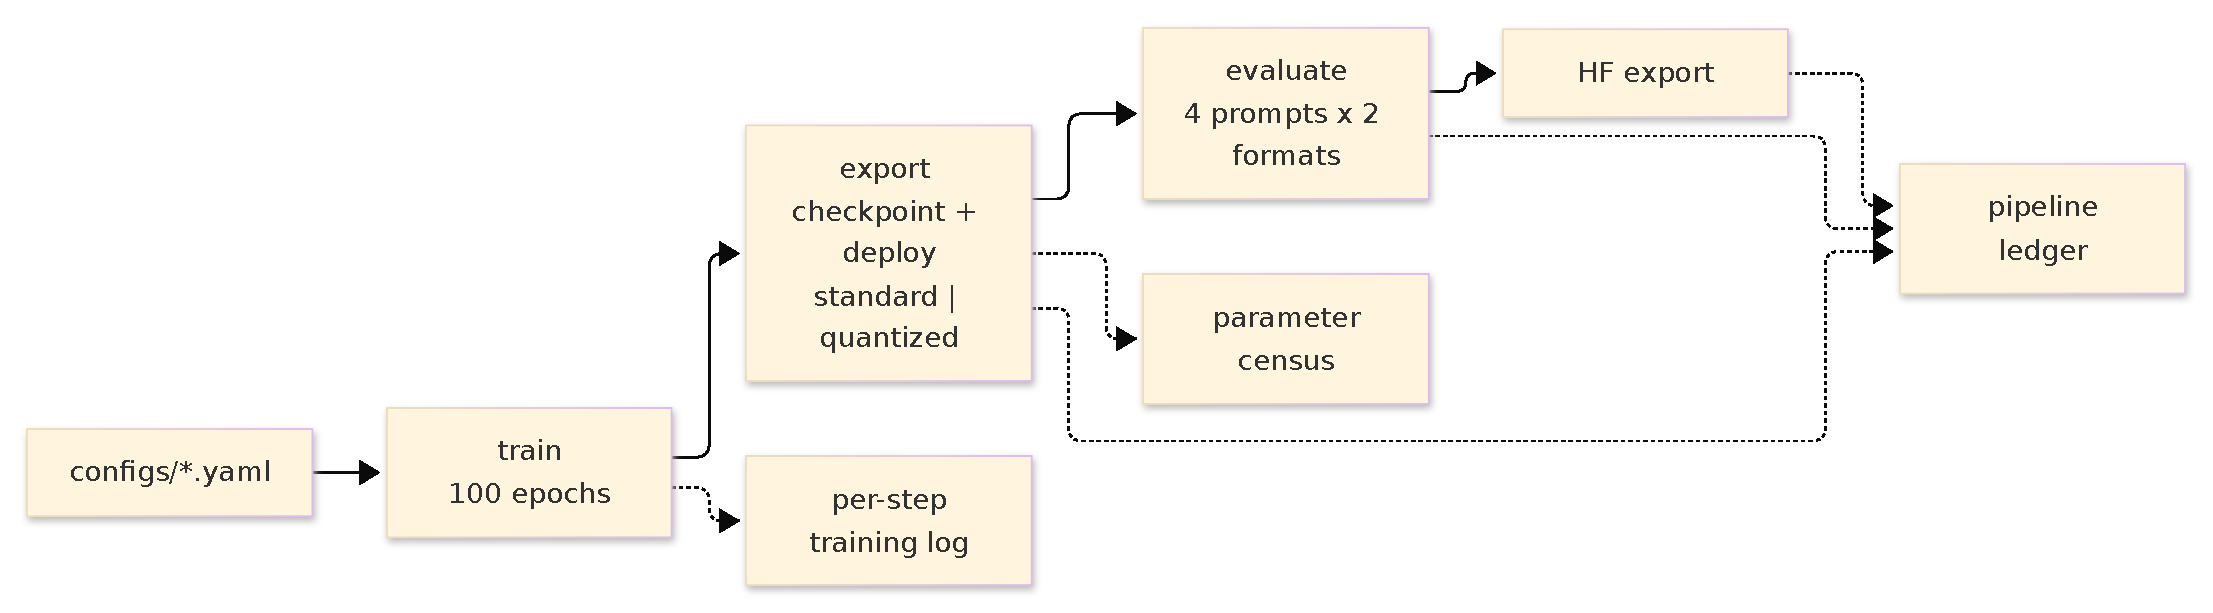
\includegraphics{../paper/figures/experiment-pipeline.pdf}}
\caption{Una configuración de una ronda. Las cinco etapas las gobierna un único archivo YAML y las registran tres registradores independientes; la cadena de reporte offline que convierte los logs en el informe publicado se documenta en el Apéndice~\ref{sec:annex-experiment-harness}.}
\label{fig:experiment-pipeline}
\end{figure}

La ronda~2 se generó programáticamente. Los pares híbridos son las combinaciones de la lista de 42 mezcladores tomadas de dos en dos, materializadas como un modelo de dos capas cuya capa~0 ejecuta el mezclador~A y la capa~1 el mezclador~B; los singles usan una sola capa. Como las combinaciones siguen el orden fijo de la lista, no existe ningún par invertido $(B, A)$, así que la asimetría ``primer versus segundo mezclador'' que se reporta abajo está confundida con el orden de la lista y debe leerse de forma descriptiva. La Tabla~\ref{tab:round2-families} resume la población.

\begin{table}[H]
\centering
\small
\caption{Población de la ronda~2. Las medianas se calculan por familia; la métrica de validación es top-1 para los pares MLM y precisión para las familias de visión, audio y datos reales.}
\label{tab:round2-families}
\begin{tabular}{lrrrrrr}
\toprule
Familia & Configs & Parám. med. & Pérd. med. & Métrica med. & tok/s med. & Min med. \\
\midrule
Pares híbridos     & 703 & 220\,928 & 9,591 & 4,08\%  & 356 & 75,3 \\
Singles            & 38  & 157\,584 & 9,762 & 3,57\%  & 366 & 24,8 \\
ViT                & 48  & 315\,694 & 1,205 & 75,97\% & 23  & 9,4  \\
Optimizadores      & 23  & 210\,752 & 10,404 & 7,76\% & 391 & 21,2 \\
Estructurales     & 20  & 210\,752 & 10,397 & 5,71\% & 387 & 21,2 \\
Codif. posicional  & 12  & 210\,752 & 10,381 & 7,76\% & 402 & 21,9 \\
Normalización      & 6   & 210\,512 & 10,348 & 1,61\% & 407 & 20,7 \\
Datos reales       & 6   & 247\,788 & 1,060 & 39,04\% & 392 & 7,6  \\
Tarea              & 4   & 210\,752 & 8,603 & 5,90\% & 457 & 19,4 \\
Tokenizer          & 4   & 210\,752 & 5,978 & 4,37\% & 4\,202 & 1,1 \\
Tamaño de lote     & 2   & 210\,752 & 10,368 & 5,40\% & 596 & 13,0 \\
BitNet/GGUF        & 1   & 209\,856 & 10,369 & ---    & 562 & ---  \\
Audio              & 1   & 147\,171 & 1,099 & 0,00\%  & 31\,082 & 1,2 \\
\bottomrule
\end{tabular}
\end{table}

\subsection{Hallazgos}

\textbf{El segundo mezclador es la palanca más fuerte.} Entre los pares híbridos, el segundo mezclador mueve la pérdida final media desde 9,37 nats (\texttt{sparsek}) hasta 10,18 (\texttt{mamba}), una brecha de 0,81 nats, mientras que el primero solo abarca 0,55 (9,26--9,81 nats, restringido a las familias con suficientes muestras). Leído columna a columna, un buen B mantiene casi todo A en la banda de 8,9--9,6 nats; leído fila a fila, ningún primer mezclador rescata a un segundo malo. A esta escala, la elección de B domina a la de A por un factor de aproximadamente 1,5$\times$.

\textbf{Emparejar no es aditivo.} Si se define la sinergia de un par como la media de sus dos marginales menos su pérdida medida, $S_{A,B} = (\mu_A + \mu_B)/2 - L_{A,B}$, la mejor interacción es \texttt{nsa+engram} con $+1{,}304$ nats y la peor \texttt{gqa+tucker} con $-1{,}018$. La cola positiva empareja un primer mezclador barato y estable con un segundo de memoria pesada; la cola negativa está dominada por segundos mezcladores que parecen promedio en aislamiento (\texttt{gta}, \texttt{gqa}, \texttt{tucker}) pero chocan al apilarse tras un A fuerte. El ruido de interacción ($\pm 0{,}3$ nats) es mayor que la diferencia entre la mayoría de los optimizadores de la ablación.

\textbf{La escala es una palanca débil a este tamaño.} Sobre los pares híbridos, el número de parámetros correlaciona con la pérdida final a $r = -0{,}20$ y con la precisión de validación a $r = -0{,}07$, mientras que predice el coste de forma fiable ($r = 0{,}68$ con el tiempo por paso, $r = 0{,}65$ con el tiempo total). El modelo más grande (\texttt{engram\_\_conformer\_attn}, 415\,904 parámetros) no es el mejor. Sobre las 868 filas la correlación parece más fuerte ($r = -0{,}43$ para la pérdida), pero eso es una confusión de familias: los transformers de visión son a la vez más grandes y mucho más fáciles de ajustar, así que la comparación de interés es la de los pares.

\textbf{La cuantización post-entrenamiento es prácticamente gratis.} De las 810 configuraciones desplegadas en ambos formatos, 800 conservan una tasa top-5 idéntica; el top-1 medio pasa de 5,62\% a 5,43\% y el top-5 medio de 13,36\% a 13,24\%, ambos deltas dentro de una muestra de evaluación. El despliegue cuantizado \emph{no} es más rápido de extremo a extremo (32,3\% de las corridas, ratio mediano 0,64$\times$) porque la etapa está dominada por la serialización y la conversión; la evaluación en sí es más rápida en el 51,2\% de las corridas con una mediana de 1,03$\times$.

\textbf{La tanda es honesta con sus fallos y sus puntos ciegos.} El libro contiene 5{,}271 registros de etapas con 275 fallos (171 de entrenamiento, 104 de despliegue), todos fuera de las 868 configuraciones analizadas. Cuatro mezcladores (\texttt{cca}, \texttt{ccgqa}, \texttt{msa}, \texttt{ssog}) nunca entrenan, lo que explica exactamente las 158 celdas ausentes del atlas de 861 celdas. Otros cuatro (\texttt{standard}, \texttt{bigbird}, \texttt{longformer}, \texttt{titan}) producen pérdidas bit a bit idénticas porque sus ventanas (al menos 64 tokens) cubren toda la secuencia de 32 tokens; el atlas mide un mismo modelo cuatro veces. Por separado, 37 pares aparecen bajo las grafías \texttt{retnet} y \texttt{retnet\_attn} con métricas idénticas, una implementación duplicada que el análisis colapsa.

\textbf{El bloque de visión funciona.} La segmentación alcanza 90,7\% de precisión media de validación, la clasificación 75,8\% y la predicción de parches 69,9\%, un orden de magnitud por encima de los pares MLM. Esa brecha refleja la dificultad de la tarea, no la calidad del mezclador, y por eso las familias se mantienen separadas en todo el informe.

\subsection{Amenazas a la validez}

El modelo es pequeño (127k--416k parámetros, un vocabulario español de 512 tokens, secuencias de 32 tokens, una semilla por configuración y 100 épocas). Todas las curvas de aprendizaje siguen bajando en la época~100, así que el ranking premia a los que aprenden rápido y no a la calidad convergida. La inferencia usa cuatro frases por configuración, de modo que un acierto extra mueve una tasa top-5 en 25 puntos porcentuales; la señal de validación es un detector de fallos catastróficos, no un instrumento de ranking. Varios optimizadores convergen a la misma pérdida porque la corrida es demasiado corta para separarlos, y una corrida de clasificación de texto colapsó a una predicción constante, lo que es un modo de fallo y no un buen modelo. Los rankings del Apéndice~\ref{sec:annex-experiment-2} son, por tanto, direccionales. La próxima ronda debería repetir el atlas con 256--512 tokens, un conjunto de evaluación de 200 frases, al menos tres semillas y 300 épocas para los mejores pares.
